% Results 

\begin{frame}{Result}


Good
	\begin{itemize}
	\item Overall great performance with one object
		\begin{itemize}
		\item Keeps track of the objects if it's not visible in the foreground
		\item No delay
		\item It's clear which safety zone the object is within
		\end{itemize}
	\item Background subtraction is reliable for moving objects
		\begin{itemize}
		\item Very little noise
		\end{itemize}
	\end{itemize}
	
	\vspace{2mm}
Slightly less good
	\begin{itemize}
	\item Performance issues with tracking
		\begin{itemize}
			\item Some delay with many objects
			\item The system sometimes loses track of objects
		\end{itemize}
	\end{itemize}	
	
\end{frame}

\begin{frame}{Conclusions}

	 \begin{columns}[c] % the "c" option specifies center vertical alignment
    \column{.5\textwidth} % column designated by a command
    
	\begin{itemize}
	\item Try other methods for object detection
	\end{itemize}
\column{.5\textwidth}
    \begin{figure}[H]
	\begin{center}
	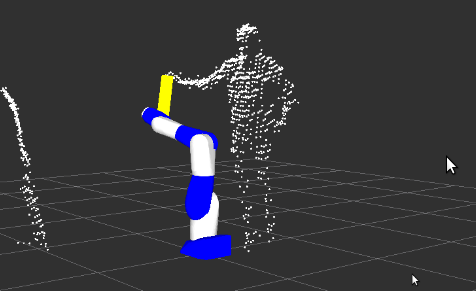
\includegraphics[width=5 cm]{resultat1}
	\end{center}
	\end{figure}
    \end{columns}

\end{frame}
